\documentclass[11pt]{article}
\usepackage[a4paper,margin=1in]{geometry}

\usepackage[T1]{fontenc}
\usepackage[utf8]{inputenc}
\usepackage{lmodern}
\usepackage{amsmath,amssymb}
\usepackage{booktabs}
\usepackage{array}
\usepackage{graphicx}
\usepackage{tikz}
\usetikzlibrary{arrows.meta,positioning,fit,backgrounds,calc,plotmarks}
\usepackage{hyperref}
\hypersetup{
  colorlinks=true,
  linkcolor=black,
  citecolor=black,
  urlcolor=blue,
  pdftitle={ReproBot -- Third Progress Report},
  pdfauthor={Aleyna Kutuk, Engincan Varan, Gul Korkut, Goktug Mert Ozdogan}
}
\usepackage{xcolor}
\usepackage{caption}
\usepackage{pifont}

\definecolor{builtc}{HTML}{1B6F50}
\definecolor{missingc}{HTML}{97303F}
\definecolor{loopc}{HTML}{0E6E78}
\definecolor{warnc}{HTML}{97590C}

\newcommand{\built}{\textcolor{builtc}{\ding{51}}}
\newcommand{\absent}{\textcolor{missingc}{\ding{55}}}
\newcommand{\partl}{\textcolor{warnc}{$\sim$}}
\newcolumntype{L}[1]{>{\raggedright\arraybackslash}p{#1}}

% Float placement: this report carries more figures and tables than the second, and
% the default fractions strand wide floats at the end of the document.
\renewcommand{\topfraction}{0.9}
\renewcommand{\dbltopfraction}{0.9}
\renewcommand{\bottomfraction}{0.8}
\renewcommand{\textfraction}{0.07}
\renewcommand{\floatpagefraction}{0.75}
\renewcommand{\dblfloatpagefraction}{0.75}
\setcounter{topnumber}{3}
\setcounter{dbltopnumber}{3}
\setcounter{totalnumber}{5}

\title{\textbf{ReproBot: A Multi-Agent System for Automated Scientific Paper Replication}\\[0.4em]
\large Third Progress Report}
\author{
  Aleyna Kütük \\ \small\texttt{aleynakutuk10@gmail.com}
  \and
  Engincan Varan \\ \small\texttt{engincanvaran@gmail.com}
  \and
  Gül Korkut \\ \small\texttt{serifegulkorkut@gmail.com}
  \and
  Göktuğ Mert Özdoğan \\ \small\texttt{goekmeroz@gmail.com}
}
\date{inzva AI Projects \#10 \\ 13.09.2026}


\begin{document}

\maketitle

\begin{abstract}
ReproBot is a multi-agent system that reads a machine learning paper, extracts its claims and
experimental setup, generates an implementation, executes it in a sandbox, and repairs
execution failures through a bounded retry loop. This report covers the phase in which it
produced its first replication measurements. Full training on the project's CIFAR-10
benchmark would take weeks per paper on the available CPU, so we evaluated on papers whose
original experiments run in minutes, and generalized code generation beyond image
classification: the Coder now writes a plain PyTorch training loop for neural models and a
scikit-learn estimator for classical ones, under a task-agnostic metrics contract. Five papers
--- a network with a margin-based loss, a tabular regression network, a kernel support vector
machine, a random forest and a soft decision tree --- were carried through the pipeline and
compared against their published claims by hand. Three reproductions land close to their
claims: an MNIST network at 0.82\% test error against 0.87\%, after one unstated
hyperparameter was corrected by hand; a support vector machine at 96.63\% against 96.9\%, whose
implementation reproduces the paper's exact numbers when given the paper's settings; and a
random forest at 87.73\% against 87.3\%. A housing-price model misses its claim, with a test
RMSE of 4.48 against 3.02, by a margin a single data split cannot explain, and a soft decision
tree whose paper states little beyond its depth did not learn at all. The retry loop repaired
three naturally occurring defects, and six prompt failures observed in real runs became
explicit rules. The central finding is that the pipeline reported \emph{success} on two runs
that had failed entirely: nothing yet judges whether a reproduced number is plausible, which
makes an automated Critic the most important missing component. We also describe the team's
first front end, a dashboard over the pipeline's outputs.
\end{abstract}

\section{Introduction}
\label{sec:intro}

Reproducing a machine learning paper's reported results is mechanical in principle and
laborious in practice, and most published work ships no usable implementation. ReproBot
automates the process as a pipeline of specialized stages. A vision-language model converts
the paper's PDF into Markdown, reading figures as well as text. A Reader extracts five
structured fields --- a method summary, architecture notes, the paper's claimed results, its
hyperparameters and its data pipeline --- and cross-checks them with a validation loop. A Coder
turns that extraction into a self-contained training script. A Runner executes the script
inside a Docker container through four escalating stages: \texttt{probe}, a few optimizer
steps; \texttt{smoke}, one epoch on a small slice; \texttt{capped}, five epochs on a small
slice; and \texttt{full}, the paper's own setup. When a stage fails, a cheap model classifies
the failure, and an Orchestrator feeds that diagnosis back to the Coder and retries, within a
fixed budget. The planned final stage, a Critic that compares each reproduced number with the
paper's claim under an explicit tolerance, does not yet exist.

At the start of this phase the pipeline could execute generated code end to end, but it had
produced no replication result. Every run on its CIFAR-10 target papers had been a short
execution check, because a full training run on the available CPU was measured at roughly
three weeks per paper. This phase changed that in three ways. Section~\ref{sec:direction}
describes a change of direction: evaluating on papers small enough to train for real on a CPU,
and a team decision that ReproBot must handle several kinds of paper and several model
families. Section~\ref{sec:generalization} describes the resulting changes to the Coder and
Runner, and Section~\ref{sec:prompts} the prompt failures that real runs exposed and the rules
that now prevent them. Section~\ref{sec:results} reports the measurements, including a
training collapse, the ablation that explained it, and five comparisons against published
claims. Section~\ref{sec:viewer} describes the team's pipeline viewer, and
Sections~\ref{sec:findings}--\ref{sec:conclusion} collect the engineering findings, methodology,
progress against plan, limitations and next steps.

Table~\ref{tab:status} summarizes the open problems at the start of the phase and where each
now stands.

\begin{table}[tbp]
\centering
\small
\caption{Open problems at the start of this phase, and their status now.}
\label{tab:status}
\begin{tabular}{L{0.34\textwidth}L{0.58\textwidth}}
\toprule
At the start of the phase & Now \\
\midrule
No reproduced number had ever been compared with a claim
  & Five claims measured at full fidelity and compared by hand
    (Section~\ref{sec:fidelity}); the Critic still does not exist \\
Full-fidelity runs infeasible ($\sim$22 days per CIFAR-10 paper)
  & Unchanged for CIFAR-10; sidestepped with CPU-sized papers whose full runs take between
    one minute and one hour \\
Only CIFAR-10 image classifiers, all built with HuggingFace \texttt{Trainer}
  & Seven papers carried end to end, spanning CNNs, MLPs, a regression network, a kernel SVM,
    a random forest and a soft decision tree \\
The retry loop had repaired only a deliberately injected fault
  & Three naturally occurring defects repaired (Section~\ref{sec:wijaya}) \\
Four of seven Orchestrator verdicts never observed in a real run
  & \texttt{environment\_error} occurred in a real run --- wrongly assigned, and the
    triage prompt corrected (Section~\ref{sec:prompts}); three remain unobserved \\
Retries regenerate whole scripts rather than patching them
  & Unchanged, and now measured: one-line fixes produced scripts only 22--27\% similar to their
    predecessors \\
Reader validation never converged; two CIFAR-10 papers cannot be extracted
  & Two papers now converge with no flags left; the rest unchanged \\
\bottomrule
\end{tabular}
\end{table}

\section{A Change of Direction}
\label{sec:direction}

\subsection{The compute wall}

The CIFAR-10 papers chosen as ReproBot's first targets are the natural benchmark for the
proposal's image-classification scope, and they are unreachable on the hardware available to
the project. At the measured throughput of 5.3 training samples per second, one
\emph{Wide Residual Networks} run at the paper's own setup takes approximately 22 days. Every number previously produced for these papers therefore came from short execution checks
that train for one epoch on a few hundred images, and could say nothing about fidelity.

Securing GPU compute remains necessary for that benchmark. It is not, however, necessary to
test the claim ReproBot actually makes --- that a paper can be read, implemented, executed
and checked automatically --- which requires only a paper whose original experiment is
small. We therefore looked for papers whose headline result trains in minutes on a CPU,
while leaving the curated CIFAR-10 set untouched.

\subsection{More than one kind of paper}

The search surfaced a structural problem. The pipeline was, in practice, hardwired to image
classification: the Coder's prompt assumed \texttt{torchvision} datasets and the HuggingFace
\texttt{Trainer} image-model interface, the metrics contract was keyed on accuracy, and the
Runner's image carried no tabular libraries. An in-scope MNIST paper would have tested the
pipeline as it stood. A housing-price regression paper could not have run at all.

The team's decision was that this was a defect rather than a scope boundary: a system that
replicates only one task type is not a general replication system, and ReproBot should
handle several. CIFAR-10 remains the main evaluation set, but no stage may now assume
images. Both candidate papers were retained, precisely because they differ:

\begin{itemize}
  \item \textbf{Tang (2013)}, \emph{Deep Learning using Linear Support Vector Machines}
    \cite{tang2013dlsvm}. A classification paper whose contribution is a loss: the softmax
    output layer is replaced by a linear L2-SVM trained with a squared hinge loss. The
    targeted claim is 0.87\% MNIST test error. The setup --- PCA to 70 dimensions, two
    512-unit hidden layers, 400 epochs --- is stated in unusual detail, which makes the two
    values it omits all the more consequential (Section~\ref{sec:tang}).
  \item \textbf{Wijaya (2023)}, \emph{Multi Level Dense Layer Neural Network Model for
    Housing Price Prediction} \cite{wijaya2023housing}. A tabular regression paper in Keras,
    on the Boston Housing data \cite{harrison1978hedonic}: 506 rows, 13 features, a stated
    405/101 train/test split, 1000 epochs. The targeted claim is a test RMSE of 3.02. It
    tests three things CIFAR-10 cannot: a non-image data source, a regression metric where
    lower is better, and a paper written for a different framework.
\end{itemize}

A replication system should also handle the models much of applied machine learning still
relies on: kernel methods, decision trees and ensembles. Three further papers were therefore
chosen to cover model families rather than tasks:

\begin{itemize}
  \item \textbf{Hsu, Chang and Lin (2003)}, \emph{A Practical Guide to Support Vector
    Classification} \cite{hsu2003guide}. A widely used tutorial whose worked examples report
    exact accuracies from the LIBSVM tools \cite{chang2011libsvm}. The target is its
    astroparticle-physics example, svmguide1 (3,089 training and 4,000 test instances, four
    features): 96.9\% test accuracy after scaling each feature to $[-1, 1]$ and choosing the
    RBF kernel's $C$ and $\gamma$ by a cross-validated grid search. Its appendix gives the
    unrounded value, 96.875\%, at $C = \gamma = 2$.
  \item \textbf{Xiao, Rasul and Vollgraf (2017)}, \emph{Fashion-MNIST}
    \cite{xiao2017fashion}. A dataset paper whose benchmark table evaluates about 130
    configurations of 13 scikit-learn classifiers \cite{pedregosa2011sklearn}. The target is
    its random forest (100 trees, entropy criterion, maximum depth 100): 0.873 test accuracy,
    the mean of five runs with shuffled training data.
  \item \textbf{Frosst and Hinton (2017)}, \emph{Distilling a Neural Network Into a Soft
    Decision Tree} \cite{frosst2017soft}. A binary tree whose inner nodes are learned linear
    filters, trained by gradient descent. The target is 94.45\% MNIST test accuracy for a
    depth-8 tree trained on true labels. The paper states the depth and little else --- no
    learning rate, batch size, epoch count, penalty strength or temperature --- so this target
    deliberately tests how the pipeline behaves when an experiment is under-specified.
\end{itemize}

Table~\ref{tab:targets} summarizes the five targets. All were kept in a separate directory,
so the curated CIFAR-10 set remains exactly as its curator left it.

\begin{table}[tbp]
\centering
\small
\caption{The five CPU-sized replication targets of this phase.}
\label{tab:targets}
\begin{tabular}{L{0.25\textwidth}L{0.22\textwidth}L{0.22\textwidth}L{0.2\textwidth}}
\toprule
Paper & Model family & Data & Targeted claim \\
\midrule
Tang (2013) & MLP with an L2-SVM output layer & MNIST & 0.87\% test error \\
Wijaya (2023) & Multi-branch dense network (Keras) & Boston Housing, tabular & Test RMSE 3.02 \\
Hsu, Chang and Lin (2003) & RBF support vector machine & svmguide1, tabular & 96.9\% test accuracy \\
Xiao et al.\ (2017) & Random forest (scikit-learn) & Fashion-MNIST & 0.873 test accuracy, 5 runs \\
Frosst and Hinton (2017) & Soft decision tree & MNIST & 94.45\% test accuracy \\
\bottomrule
\end{tabular}
\end{table}

\section{Generalizing the Coder and Runner}
\label{sec:generalization}


\begin{figure}[tbp]
\centering
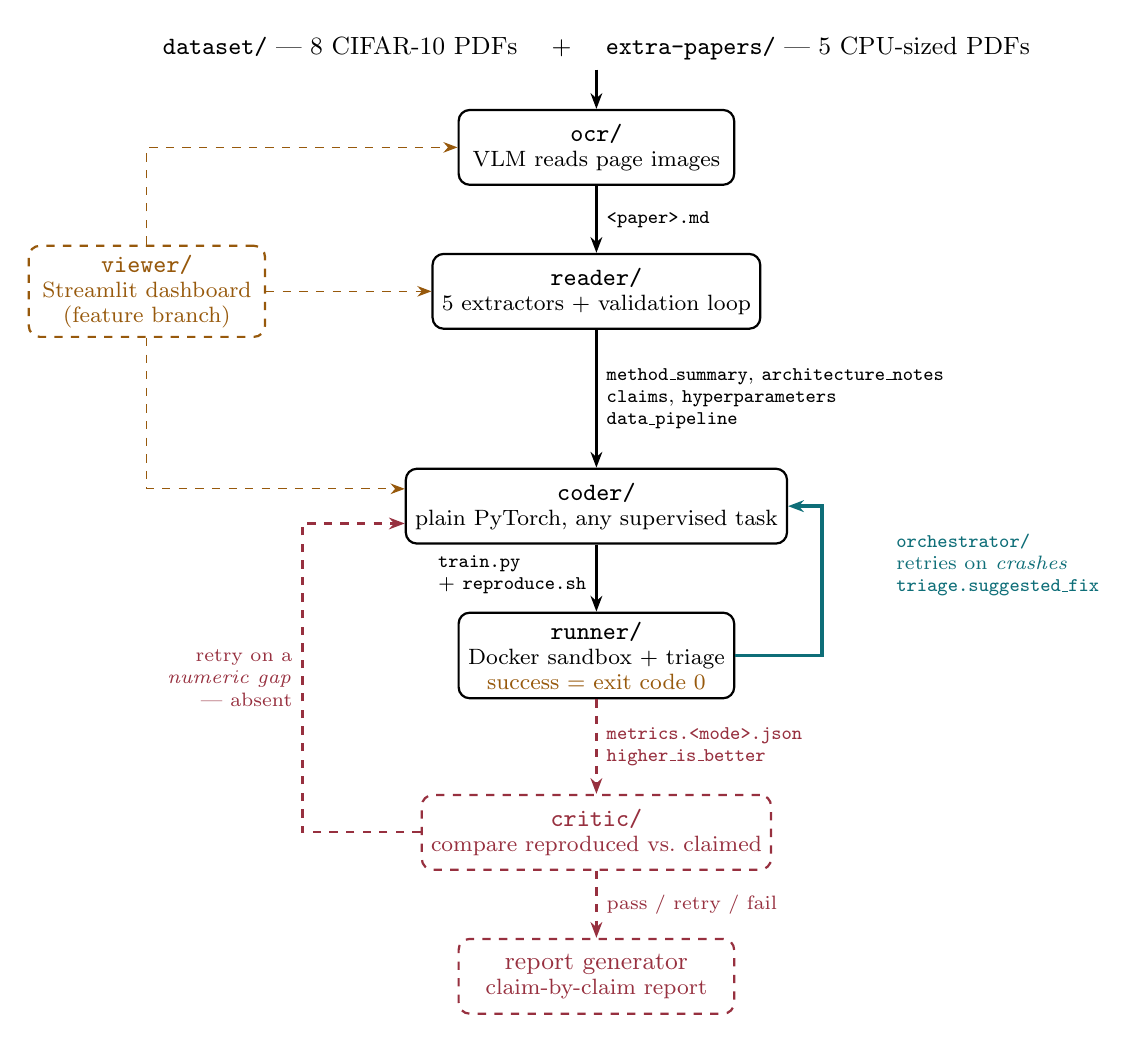
\begin{tikzpicture}[
  node distance=0.85cm and 1.5cm,
  stage/.style={draw, rounded corners, minimum width=3.5cm, minimum height=0.95cm,
    align=center, font=\small, thick},
  gone/.style={draw, rounded corners, minimum width=3.5cm, minimum height=0.95cm,
    align=center, font=\small, dashed, thick, draw=missingc, text=missingc},
  side/.style={draw, rounded corners, minimum width=3.0cm, minimum height=0.95cm,
    align=center, font=\small, thick, dashed, draw=warnc, text=warnc},
  arr/.style={-{Stealth[length=2mm]}, thick},
  gonearr/.style={-{Stealth[length=2mm]}, thick, dashed, draw=missingc},
  sidearr/.style={-{Stealth[length=1.8mm]}, dashed, draw=warnc},
  looparr/.style={-{Stealth[length=2mm]}, very thick, draw=loopc},
  lbl/.style={font=\scriptsize, align=left},
  gonelbl/.style={font=\scriptsize, align=left, text=missingc}
]
  \node[stage] (ocr)    {\texttt{ocr/}\\[-2pt]\footnotesize VLM reads page images};
  \node[stage, below=of ocr] (reader) {\texttt{reader/}\\[-2pt]\footnotesize 5 extractors + validation loop};
  \node[stage, below=1.75cm of reader] (coder) {\texttt{coder/}\\[-2pt]\footnotesize plain PyTorch, any supervised task};
  \node[stage, below=of coder] (runner) {\texttt{runner/}\\[-2pt]\footnotesize Docker sandbox + triage\\[-2pt]\footnotesize\textcolor{warnc}{success = exit code 0}};
  \node[gone,  below=1.2cm of runner] (critic) {\texttt{critic/}\\[-2pt]\footnotesize compare reproduced vs.\ claimed};
  \node[gone,  below=of critic] (report) {report generator\\[-2pt]\footnotesize claim-by-claim report};

  \node[above=0.5cm of ocr, font=\small, align=center] (pdf)
    {\texttt{dataset/} --- 8 CIFAR-10 PDFs \quad $+$ \quad \texttt{extra-papers/} --- 5 CPU-sized PDFs};

  \node[side, left=2.1cm of reader] (viewer) {\texttt{viewer/}\\[-2pt]\footnotesize Streamlit dashboard\\[-2pt]\footnotesize (feature branch)};
  \draw[sidearr] (viewer.north) |- (ocr.west);
  \draw[sidearr] (viewer.east) -- (reader.west);
  \draw[sidearr] (viewer.south) |- ([yshift=0.22cm]coder.west);

  \draw[arr] (pdf) -- (ocr);
  \draw[arr] (ocr) -- node[right, lbl] {\texttt{<paper>.md}} (reader);
  \draw[arr] (reader) -- node[right, lbl]
    {\texttt{method\_summary}, \texttt{architecture\_notes}\\
     \texttt{claims}, \texttt{hyperparameters}\\ \texttt{data\_pipeline}} (coder);
  \draw[arr] (coder) -- node[left, lbl, pos=0.45] {\texttt{train.py}\\ + \texttt{reproduce.sh}} (runner);
  \draw[gonearr] (runner) -- node[right, gonelbl] {\texttt{metrics.<mode>.json}\\ \texttt{higher\_is\_better}} (critic);
  \draw[gonearr] (critic) -- node[right, gonelbl] {pass / retry / fail} (report);

  \draw[looparr] (runner.east) -- ++(1.1,0) |- (coder.east);
  \node[lbl, text=loopc, right=1.25cm of coder.east, anchor=west, yshift=-0.75cm]
    {\textbf{\texttt{orchestrator/}}\\ retries on \emph{crashes}\\ \texttt{triage.suggested\_fix}};

  \draw[gonearr] (critic.west) -- ++(-1.5,0) |- node[pos=0.25, left, gonelbl, align=right]
    {retry on a\\ \emph{numeric gap}\\ --- absent} ([yshift=-0.22cm]coder.west);
\end{tikzpicture}
\caption{ReproBot on 13.09.2026. Solid components are built and verified by execution;
dashed red components do not exist; the dashed amber component is on a feature branch. The
pipeline's shape predates this phase, but its inputs now include CPU-sized papers beyond
image classification, and the Coder writes a plain PyTorch loop or a scikit-learn estimator
depending on the paper's model family. The label inside the Runner marks this phase's central finding: a run is
reported as a success when its script exits normally, whatever number it produced.}
\label{fig:pipeline}
\end{figure}


\subsection{Dropping the HuggingFace \texttt{Trainer}}

The Coder previously emitted scripts built on HuggingFace's \texttt{Trainer}. Its model
contract --- image tensors in, logits out --- fits a custom margin loss or a regression head
poorly, and that alone argued for replacing it. The deciding reason, however, was that
\texttt{Trainer} applies defaults that no paper states, and this was demonstrated rather than
assumed.

When the generalized Coder regenerated its \emph{Network In Network} script as a regression
test, the new plain-PyTorch script kept the paper's architecture --- a genuine
\texttt{mlpconv} cascade with no fully-connected layer --- and passed its execution probe.
But its loss reached approximately 947, where the previous \texttt{Trainer}-based script had
reported 2.30. The cause was a default: the old script never set \texttt{max\_grad\_norm},
and therefore inherited \texttt{Trainer}'s gradient clipping at a norm of 1.0, which we
confirmed inside the container. The paper uses no clipping. Faithful to the paper and without
its unstated initialization, the same learning rate diverges.

This changes how earlier results should be read. The \emph{Network In Network} runs made
before this change executed under a stabilizing mechanism the paper does not describe. Their
numbers had only ever been treated as execution checks, not replication results, but the
scripts that produced them were less faithful to the paper than they appeared. The Coder is now forbidden from using \texttt{Trainer}, \texttt{accelerate},
Lightning or Keras, and writes an explicit training loop in which every mechanism is visible.

\subsection{Always PyTorch, whatever the paper used}

Wijaya's model was built in Keras. Rather than generate code for a second framework, the
Coder always writes PyTorch, and the prompt treats the source framework's defaults as part of
the method: where a paper is silent, it inherited its framework's behaviour, so a faithful
translation must reproduce that behaviour. The prompt names the Keras defaults that differ ---
Adam's $\epsilon = 10^{-7}$, Glorot initialization, batch normalization with momentum 0.99 and
$\epsilon = 10^{-3}$, and a \texttt{fit()} batch size of 32 --- and requires every remaining
difference to be disclosed. Section~\ref{sec:findings} reports that this rule was followed
only in part.

\subsection{A task-agnostic metrics contract}

Every generated script writes a fixed-shape metrics file that the Runner parses and a future
Critic will read. The original contract was designed for image classification and assumed accuracy. Its
generalization is summarized in Table~\ref{tab:contract}; the most consequential addition is
\texttt{higher\_is\_better}, since a bare value of 4.0 is meaningless without knowing
whether it is an error or an accuracy.

\begin{table}[tbp]
\centering
\small
\caption{Changes to the metrics contract. \texttt{metric} and \texttt{unit} are copied
verbatim from the targeted claim, so a comparison against the claim needs no conversion.
Files in the old shape still parse.}
\label{tab:contract}
\begin{tabular}{L{0.36\linewidth}L{0.54\linewidth}}
\toprule
Field & Change \\
\midrule
\texttt{train\_metric}, \texttt{eval\_metric} & Replace \texttt{train\_accuracy} and
  \texttt{eval\_accuracy}: the claim's own metric on each split \\
\texttt{higher\_is\_better} & New; the direction of the metric \\
\texttt{task\_type} & New; inferred by the Coder from the claim, e.g.\
  \texttt{classification} or \texttt{regression} \\
\texttt{value}, \texttt{metric}, \texttt{unit} & Unchanged; the headline number and its
  claim-verbatim label \\
\bottomrule
\end{tabular}
\end{table}

\subsection{Data sourcing, and verifying what was fetched}

Image datasets still come from \texttt{torchvision}. Tabular data is fetched from OpenML,
pinned by dataset identifier, before any direct URL is considered, and every download lands
in the shared dataset cache the Runner mounts. The preference order was not a design choice
made in advance; Section~\ref{sec:prompts} describes the failure that produced it.

The generated script must also check, in code and before training, that the dataset it
fetched is the one it intended --- its name, row count and column count --- and raise
otherwise. The motivation is that a wrong identifier does not fail. It downloads a different
dataset that happens to carry that number, trains on it, and reports a plausible metric for
the wrong problem. Where a paper gives split sizes but not how the split was drawn, the
script uses a seeded random split and records the assumption.

\subsection{Classical estimators in scikit-learn}

Writing everything in PyTorch is right for neural networks and wrong for everything else.
Re-implementing a support vector machine as a PyTorch model trained by stochastic gradient
descent on a hinge loss changes both the optimizer and the solution it reaches; a paper that
ran LIBSVM ran a specific quadratic-programming solver. The Coder therefore now chooses its
library by model family. Classical estimators --- support vector machines, decision trees and
forests, $k$-nearest neighbours, logistic regression, naive Bayes and similar --- are built with
scikit-learn, whose \texttt{SVC} wraps LIBSVM itself, with every hyperparameter passed
explicitly by name. Neural models stay in PyTorch, including tree-shaped models trained by
gradient descent, such as a soft decision tree.

Three further rules let this work without changing the Runner. First, library versions ship
different defaults, just as frameworks do: before scikit-learn 0.22 a random forest defaulted
to 10 trees and an RBF \texttt{SVC} to $\gamma = 1/n_{\text{features}}$, and a paper that relied
on defaults relied on those. The Coder sets the paper-era values explicitly and discloses each
one. Second, the command-line contract every generated script must satisfy is unchanged: flags
with no meaning for an estimator, such as a learning rate for a random forest, are accepted as
documented no-ops, while the sample caps that make the cheap stages cheap still apply, and loss
and epoch fields in the metrics file may be empty. Third, when a claim is an average over
repeated runs or cross-validation folds, the full run performs every repetition and reports the
mean alongside the per-run values, while the cheap stages run a single repetition.

\subsection{Runner changes}

The Runner's interface did not change: it still invokes only the generated
\texttt{reproduce.sh} and one of its four modes, which is what allowed new task types and model
families to be added without modifying its code. Classical estimators needed no Runner change
at all. Its image gained pinned \texttt{pandas},
\texttt{scikit-learn} and \texttt{scipy}, installed in the same \texttt{pip} command as the
pinned \texttt{numpy}, so that a transitive upgrade fails the build rather than silently
moving a numerical dependency.

\section{Prompt Hardening from Real Failures}
\label{sec:prompts}

Running the generalized pipeline on real papers exposed six failures in the prompts of the
Coder and of the Runner's triage step. None was found by inspection; each surfaced in a run.
Table~\ref{tab:prompts} lists them with the rule that now addresses each. Every triage rule
was verified by re-running triage on the real log that exposed the problem.

\begin{table}[tbp]
\centering
\small
\caption{Prompt failures observed in real runs, in the order they occurred, and the rule
that now addresses each. Rows 1--5 arose from the first tabular run; row 6 from its rerun.}
\label{tab:prompts}
\begin{tabular}{r L{0.33\textwidth} L{0.23\textwidth} L{0.31\textwidth}}
\toprule
& Observed failure & Consequence & Rule now in the prompt \\
\midrule
1 & The Coder fetched Boston Housing from a remembered CMU StatLib URL, which now returns
    HTTP~403 to every client
  & The first execution stage failed in 5\,s
  & Coder: OpenML by identifier first; a direct URL only for data found nowhere else \\
2 & Triage classified the 403 as \texttt{environment\_error}
  & The Orchestrator stopped with zero retries on a failure one regeneration would fix
  & Triage: a refusal from one source is recoverable; only a container with no network at
    all is environmental \\
3 & A re-triage suggested switching to ``a standard alternative regression dataset''
  & The fix would change what is being reproduced
  & Never change what is being reproduced \\
4 & A re-triage suggested \texttt{load\_boston}
  & That loader was removed from scikit-learn in version 1.2
  & Never suggest an API or source not certainly current; give one fix, not a menu \\
5 & A re-triage named Boston Housing as OpenML \texttt{data\_id=506}
  & Identifier 506 is a different dataset (Boston Housing is 531); training would
    silently proceed on it
  & Name no identifier absent from the log; the Coder asserts the dataset's name and shape
    in code \\
6 & The Coder's prompt twice said ``OpenML data\_id and version''; the script passed both
  & \texttt{fetch\_openml} rejects that combination with a \texttt{ValueError}
  & Pin by identifier alone, or by name together with a version \\
\bottomrule
\end{tabular}
\end{table}

Two of these generalize beyond this project, and are drawn out in
Section~\ref{sec:findings}. Rows 1 and 5 share a pattern: in both, a model supplied an
identifier from memory that looked exactly as plausible as a correct one. Row 6 is the
converse, and the more uncomfortable: the defect was in our own prompt, whose descriptive
wording the model implemented literally.

\section{Results}
\label{sec:results}

\subsection{Extraction on the new papers}

The Reader ran unchanged on all five papers. Table~\ref{tab:reader} compares them with the four
CIFAR-10 papers it had already processed. Every targeted claim was extracted, as was Tang's
distinction between the L1- and L2-SVM gradients.

\begin{table}[tbp]
\centering
\small
\caption{Reader output across nine papers; the first four rows are CIFAR-10 papers processed before this phase. \emph{Comp.} is architecture components; \emph{own/eq} is equations marked as the
paper's own over equations captured; \emph{Gaps} is \texttt{unstated\_details} entries;
\emph{Flags} is unresolved validation flags after the three-pass cap.}
\label{tab:reader}
\begin{tabular}{lrrrrcrr}
\toprule
Paper & Claims & Hyp. & Data & Comp. & own/eq & Gaps & Flags \\
\midrule
Network In Network      & 12 & 17 & 4 &  7 & 1/3  & 12 & 4 \\
All Convolutional Net   & 17 & 13 & 4 & 10 & 2/6  & 11 & 5 \\
Deep Residual Learning  & 66 & 28 & 6 & 10 & 2/3  &  7 & 8 \\
Wide Residual Networks  & 61 & 20 & 4 & 11 & 1/1  & 11 & 6 \\
\midrule
Tang (2013), DLSVM      & 15 & 23 & 3 & 10 & 4/11 & 12 & 5 \\
Wijaya (2023), housing  & 14 & 10 & 1 &  8 & 2/2  &  8 & 5 \\
Hsu et al.\ (2003), SVM guide & 3 & 19 & 8 & 2 & 0/6 & 5 & 0 \\
Xiao et al.\ (2017), Fashion-MNIST & 26 & 14 & 1 & 0 & 0/0 & 3 & 0 \\
Frosst and Hinton (2017), soft tree & 8 & 11 & 3 & 4 & 5/5 & 10 & 4 \\
\bottomrule
\end{tabular}
\end{table}

Two of the classical-ML papers exposed an assumption built into the Reader. Its claims
extractor keeps only a paper's own results and discards baseline rows, which is the right rule
for a paper that proposes a method. Fashion-MNIST proposes a dataset: every row of its
benchmark table is a standard classifier. On the first pass the extractor considered 124
candidate rows and kept none, and the architecture extractor found no components. The
validator flagged the empty claims against the paper's table, and the retry kept 26 --- the
best configuration of each classifier on each dataset. The loop recovered only because the
validator noticed: a kind of paper the extractor's instructions never anticipated produced a
well-formed, empty result. The same two papers were, however, the first whose validation
converged with no flags remaining. For the SVM guide, the Reader took the rounded 96.9\% from
the paper's summary table rather than the appendix's 96.875\%, and did not record the
appendix's accuracies under default parameters as claims.

Three weaknesses surfaced on the neural-network papers, all recorded as open defects. First,
validation still does not converge there: both end with five unresolved flags. Second, the same result is
extracted two or three times when a paper states it in prose, a table and a figure;
Wijaya's 14 claims describe eight distinct results, at mixed precision (0.911 and 0.91). A
Critic comparing against claims will need them deduplicated. Third, and most consequential,
the Reader records what a paper leaves unstated only for its \emph{architecture}. Tang's
paper states ``stochastic gradient descent with momentum'' without a momentum value, and an
L2-SVM objective without its penalty constant $C$. Neither omission was flagged anywhere ---
and they are exactly the two values that collapsed training (Section~\ref{sec:tang}).

\subsection{The retry loop repairs real defects}
\label{sec:wijaya}


\begin{figure}[tbp]
\centering
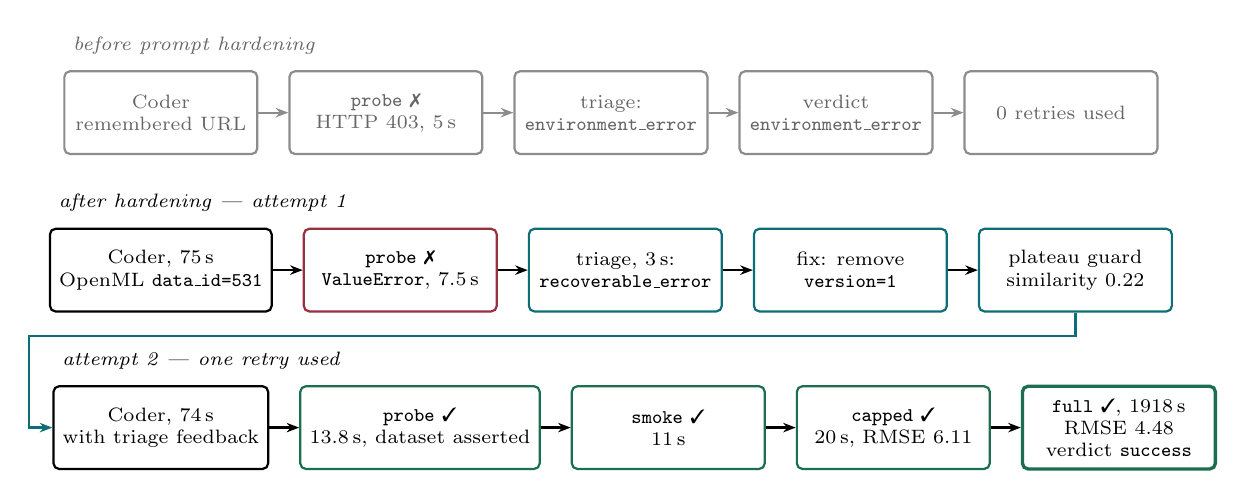
\begin{tikzpicture}[
  st/.style={draw, rounded corners=2pt, minimum width=2.45cm, minimum height=1.05cm,
    align=center, font=\scriptsize, thick},
  ok/.style={st, draw=builtc},
  bad/.style={st, draw=missingc},
  tri/.style={st, draw=loopc},
  old/.style={st, draw=black!45, text=black!60},
  arr/.style={-{Stealth[length=1.6mm]}, thick},
  row/.style={font=\scriptsize\itshape, anchor=south west}
]
  % row 0: before prompt hardening
  \node[old] (a0) at (0,0) {Coder\\ remembered URL};
  \node[old, right=0.38cm of a0] (b0) {\texttt{probe} \ding{55}\\ HTTP 403, 5\,s};
  \node[old, right=0.38cm of b0] (c0) {triage:\\ \texttt{environment\_error}};
  \node[old, right=0.38cm of c0] (d0) {verdict\\ \texttt{environment\_error}};
  \node[old, right=0.38cm of d0] (e0) {0 retries used};
  \draw[arr, black!45] (a0) -- (b0); \draw[arr, black!45] (b0) -- (c0);
  \draw[arr, black!45] (c0) -- (d0); \draw[arr, black!45] (d0) -- (e0);
  \node[row, text=black!60] at ([yshift=0.08cm]a0.north west) {before prompt hardening};

  % row 1: attempt 1
  \node[st] (a1) at (0,-2.0) {Coder, 75\,s\\ OpenML \texttt{data\_id=531}};
  \node[bad, right=0.38cm of a1] (b1) {\texttt{probe} \ding{55}\\ \texttt{ValueError}, 7.5\,s};
  \node[tri, right=0.38cm of b1] (c1) {triage, 3\,s:\\ \texttt{recoverable\_error}};
  \node[tri, right=0.38cm of c1] (d1) {fix: remove\\ \texttt{version=1}};
  \node[tri, right=0.38cm of d1] (e1) {plateau guard\\ similarity 0.22};
  \draw[arr] (a1) -- (b1); \draw[arr] (b1) -- (c1); \draw[arr] (c1) -- (d1); \draw[arr] (d1) -- (e1);
  \node[row] at ([yshift=0.08cm]a1.north west) {after hardening --- attempt 1};

  % row 2: attempt 2
  \node[st] (a2) at (0,-4.0) {Coder, 74\,s\\ with triage feedback};
  \node[ok, right=0.38cm of a2] (b2) {\texttt{probe} \ding{51}\\ 13.8\,s, dataset asserted};
  \node[ok, right=0.38cm of b2] (c2) {\texttt{smoke} \ding{51}\\ 11\,s};
  \node[ok, right=0.38cm of c2] (d2) {\texttt{capped} \ding{51}\\ 20\,s, RMSE 6.11};
  \node[ok, right=0.38cm of d2, line width=1.2pt] (e2) {\texttt{full} \ding{51}, 1918\,s\\ RMSE 4.48\\ verdict \texttt{success}};
  \draw[arr] (a2) -- (b2); \draw[arr] (b2) -- (c2); \draw[arr] (c2) -- (d2); \draw[arr] (d2) -- (e2);
  \node[row] at ([yshift=0.08cm]a2.north west) {attempt 2 --- one retry used};

  \draw[arr, draw=loopc] (e1.south) -- ++(0,-0.3) -| ([xshift=-0.3cm]a2.west) -- (a2.west);
\end{tikzpicture}
\caption{Wijaya's orchestrated runs. Top: before the prompt changes of
Section~\ref{sec:prompts}, a dead URL was classified as an environmental fault and the loop
stopped without retrying. Middle and bottom: after them, a genuine defect in the regenerated
script was triaged correctly, the Coder regenerated with the one-line fix as feedback, and
the retry passed every stage. The plateau guard's 0.22 is far below its 0.98 stopping
threshold --- and shows how much of the script changed to remove one argument.}
\label{fig:wijayarun}
\end{figure}


Until this phase, the retry loop had been demonstrated only against a deliberately
reintroduced fault: a learning-rate scheduler reading an attribute its constructor never set,
which is valid Python and fails only at run time. Wijaya's two orchestrated runs, shown in Figure~\ref{fig:wijayarun}, supply the first
naturally occurring case --- and, in the row before it, the failure that motivated the
triage rules of Section~\ref{sec:prompts}.

Before the prompts were hardened, the first execution stage failed on the dead URL, triage
called it environmental, and the loop stopped as designed for an environmental fault ---
correctly given its input, and wrongly in fact. After hardening, the regenerated script
fetched the right dataset but passed both an identifier and a version to
\texttt{fetch\_openml}, which raised. Triage classified the failure as recoverable and
proposed removing the \texttt{version} argument, which matches the traceback exactly. The
Coder regenerated with that feedback, the plateau guard measured a similarity of 0.22, and
the second attempt asserted the dataset's name and shape and passed every stage through
\texttt{full}. The whole repair cost two generation calls, one triage call, and under three
minutes.

The classical-ML and soft-tree runs added two more naturally occurring repairs. The SVM
script's cheap stages trained on the first 256 training rows; svmguide1's training file is
sorted by label, and its first 2,000 rows all belong to one class, so scikit-learn refused to
fit. Triage classified the failure as recoverable, and the regenerated script sampled the cheap
subset at random and passed every stage. The soft-tree script modified a tensor in place inside
the autograd graph, a classic PyTorch error that surfaces only in the backward pass; triage
identified the in-place operation, and the regenerated script ran. The plateau guard measured
similarities of 0.25 and 0.27 for the two regenerations.

\subsection{The first full run, and its collapse}
\label{sec:tang}

Tang's generated script passed \texttt{probe}, \texttt{smoke} and \texttt{capped} with
training error falling from 75\% to 31\% --- evidence, as far as those stages can provide
it, that the network learned. Its \texttt{full} run was ReproBot's first at a paper's own
scale. By epoch 20 its training error had risen to 83\%, and it then settled near 89.5\%
(Figure~\ref{fig:tang}). It was noticed by a team member reading the live training log. No
stage noticed, and had the run completed, the Runner would have reported \emph{success}:
the script exited normally and wrote a well-formed metrics file.


\begin{figure}[tbp]
\centering

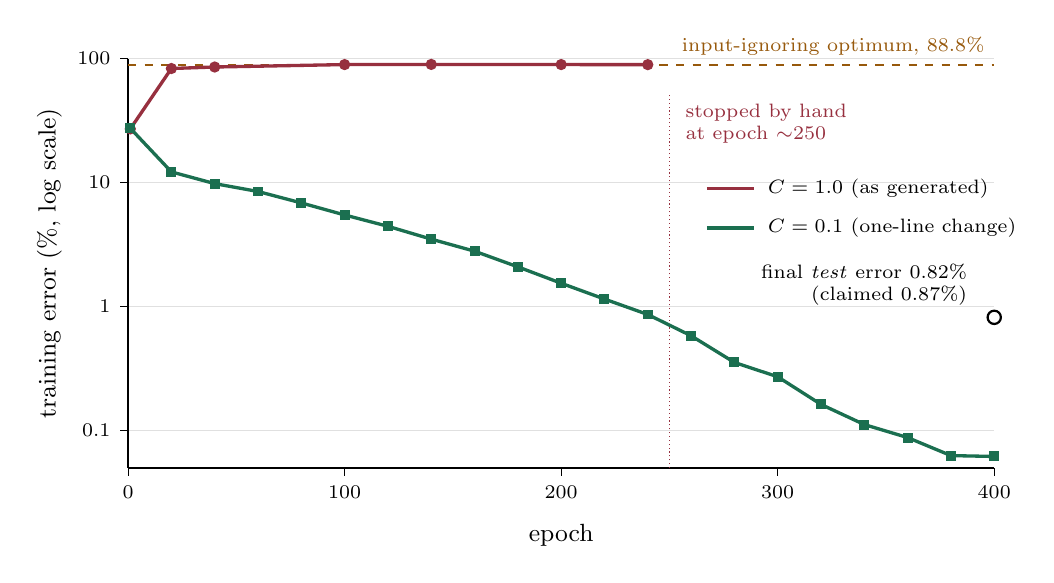
\begin{tikzpicture}[gridc/.style={draw=black!12}]
  \draw (0,0.474) -- (-0.1,0.474) node[left, font=\scriptsize] {0.1};
  \draw[gridc] (0,0.474) -- (11.0,0.474);
  \draw (0,2.049) -- (-0.1,2.049) node[left, font=\scriptsize] {1};
  \draw[gridc] (0,2.049) -- (11.0,2.049);
  \draw (0,3.625) -- (-0.1,3.625) node[left, font=\scriptsize] {10};
  \draw[gridc] (0,3.625) -- (11.0,3.625);
  \draw (0,5.200) -- (-0.1,5.200) node[left, font=\scriptsize] {100};
  \draw[gridc] (0,5.200) -- (11.0,5.200);
  \draw (0.000,0) -- (0.000,-0.1) node[below, font=\scriptsize] {0};
  \draw (2.750,0) -- (2.750,-0.1) node[below, font=\scriptsize] {100};
  \draw (5.500,0) -- (5.500,-0.1) node[below, font=\scriptsize] {200};
  \draw (8.250,0) -- (8.250,-0.1) node[below, font=\scriptsize] {300};
  \draw (11.000,0) -- (11.000,-0.1) node[below, font=\scriptsize] {400};
  \draw[thick] (0,0) -- (11.0,0);
  \draw[thick] (0,0) -- (0,5.2);
  \node[rotate=90, font=\small] at (-1.0,2.600) {training error (\%, log scale)};
  \node[font=\small] at (5.500,-0.85) {epoch};
  \draw[dashed, draw=warnc, thick] (0,5.119) -- (11.0,5.119);
  \node[font=\scriptsize, text=warnc, anchor=south east] at (11.0,5.119)
    {input-ignoring optimum, 88.8\%};
  \draw[densely dotted, draw=missingc] (6.875,0) -- (6.875,4.769);
  \node[font=\scriptsize, text=missingc, anchor=west, align=left] at (6.955,4.369)
    {stopped by hand\\ at epoch $\sim$250};
  \draw[missingc, very thick, mark=*, mark size=1.4pt]
    plot coordinates {(0.028,4.307) (0.550,5.074) (1.100,5.093) (2.750,5.124) (3.850,5.126) (5.500,5.124) (6.600,5.123)};
  \draw[builtc, very thick, mark=square*, mark size=1.2pt]
    plot coordinates {(0.028,4.315) (0.550,3.761) (1.100,3.612) (1.650,3.512) (2.200,3.367) (2.750,3.214) (3.300,3.070) (3.850,2.907) (4.400,2.754) (4.950,2.555) (5.500,2.347) (6.050,2.146) (6.600,1.950) (7.150,1.680) (7.700,1.341) (8.250,1.159) (8.800,0.808) (9.350,0.552) (9.900,0.387) (10.450,0.158) (11.000,0.147)};
  \draw[black, fill=white, thick] (11.000,1.914) circle (2.4pt);
  \node[font=\scriptsize, anchor=east, align=right] at (10.780,2.334)
    {final \emph{test} error 0.82\%\\ (claimed 0.87\%)};
  \draw[missingc, very thick] (7.35,3.55) -- (7.95,3.55);
  \node[font=\scriptsize, anchor=west] at (8.0,3.55) {$C = 1.0$ (as generated)};
  \draw[builtc, very thick] (7.35,3.05) -- (7.95,3.05);
  \node[font=\scriptsize, anchor=west] at (8.0,3.05) {$C = 0.1$ (one-line change)};
\end{tikzpicture}
\caption{Training error for Tang's reproduction at the paper's full setting, from the run
logs. As generated ($C = 1.0$, momentum 0.9), the network learned for a few epochs and then
collapsed onto the error of a network that ignores its input; the run was stopped by hand.
With the single change $C = 0.1$, training error fell smoothly to 0.062\%, and the test set,
evaluated once after the final epoch, gave 0.82\% against the claimed 0.87\%. The loss
values of the two runs are not comparable, since $C$ scales the loss, so error is plotted.}
\label{fig:tang}
\end{figure}


\textbf{Diagnosis.} For a one-vs-rest squared hinge loss, a network that ignores its input can
do no better than a constant score per class, $s_k = 2p_k - 1$, where $p_k$ is the frequency
of class $k$. The resulting loss is $\sum_k 4p_k(1-p_k)$, and the best such network always
predicts the most frequent digit. Evaluated at MNIST's class frequencies, both quantities
match the observed run (Table~\ref{tab:floor}). The network had died: early oversized
updates drove every hidden unit's pre-activation negative, so every ReLU output zero for
every input and no gradient reached the hidden layers; only the output bias still learned,
to exactly the input-ignoring optimum. A decaying learning rate cannot recover from this,
since a zero gradient stays zero at any step size.

\begin{table}[tbp]
\centering
\small
\caption{The collapsed run against a network that ignores its input. The small excess is
the L2 penalty and the input noise.}
\label{tab:floor}
\begin{tabular}{lrr}
\toprule
& Input-ignoring optimum & Observed \\
\midrule
Training loss  & 3.599 & $\sim$3.607 \\
Training error & 88.8\% & $\sim$89.5\% \\
\bottomrule
\end{tabular}
\end{table}

\textbf{Ablation.} The Coder had disclosed four values the paper does not state: momentum
0.9, $C = 1.0$, PyTorch's default initialization, and unwhitened PCA features. To isolate
the cause, we wrote a harness that imports the model, loss and data loading \emph{from the
generated script itself}, holds every paper-stated value fixed, and varies one of the four
guesses at a time for 30 epochs of the paper's schedule, measuring the fraction of hidden
units that output zero for every one of 2,000 probe images. Table~\ref{tab:ablation} reports
the six configurations.

\begin{table}[tbp]
\centering
\small
\caption{Ablation over the four unstated values, each changed alone from the generated
configuration (A). \emph{Dead} is the fraction of second-layer hidden units that output
zero for all 2,000 probe images at epoch 30; first-layer units were never dead in any
configuration.}
\label{tab:ablation}
\begin{tabular}{llrrrl}
\toprule
& Configuration & Test @5 & Test @30 & Dead @30 & Outcome \\
\midrule
A & As generated (mom.\ 0.9, $C=1.0$) & 6.6\%  & 47.1\% & 0.71 & unstable \\
B & Momentum 0.5                        & 4.0\%  & 2.62\% & 0.38 & stable \\
C & Momentum 0.0                        & 4.2\%  & 2.66\% & 0.14 & stable \\
D & $C = 0.1$                           & 4.4\%  & 2.80\% & 0.04 & stable, healthiest \\
E & PCA whitened                        & 79.8\% & 90.3\% & 0.996 & total collapse \\
F & Init.\ $\mathcal{N}(0, 0.01)$     & 5.0\% & 4.2\% & 0.31 & stable, slower \\
\bottomrule
\end{tabular}
\end{table}

The collapse requires momentum 0.9 and $C = 1.0$ \emph{together}: reducing either alone
stabilizes training. Momentum 0.9 amplifies the effective step roughly tenfold, and $C = 1.0$
scales the squared-hinge gradient tenfold relative to $C = 0.1$. Each value is a reasonable
default in isolation; the pair is too aggressive for this loss at the paper's learning rate
of 0.1. Whitening the PCA features enlarges the inputs --- the mean squared norm rises from
46 to 70 --- and collapses fastest, which supports the Coder's literal, unwhitened reading.
Configuration A degraded but did not fully collapse within 30 epochs while the real run did;
the two used different random streams for the input noise, so the collapse is
seed-dependent, which is precisely what makes it hard to catch with short runs.

We selected $C = 0.1$ (configuration D) as a one-line change to the existing script rather
than a regeneration, so that nothing else could change at the same time. It keeps the
momentum consistent with the paper's ``with momentum'', produced the healthiest network, and
concerns a constant the paper itself treats as tuned elsewhere.

\subsection{First fidelity measurements}
\label{sec:fidelity}

All five papers completed their check stages, and four completed \texttt{full} runs at their
papers' stated settings. Table~\ref{tab:fidelity} reports the results against the published
claims.

\begin{table}[tbp]
\centering
\small
\caption{ReproBot's first full-fidelity measurements, compared against the claims by hand.
Runtimes are the full stage's wall clock on the development CPU; some runs shared it.}
\label{tab:fidelity}
\begin{tabular}{L{0.16\textwidth}L{0.15\textwidth}rrrL{0.25\textwidth}}
\toprule
Paper & Claim & Claimed & Reproduced & Runtime & Reading \\
\midrule
Tang (2013) & MNIST test error & 0.87\% & \textbf{0.82\%} & 3,223\,s
  & Consistent with the claim, after one unstated value was corrected by hand \\
Wijaya (2023) & Test RMSE & 3.02 & \textbf{4.48} & 1,918\,s
  & Not reproduced on this split \\
Wijaya (2023) & Train RMSE & 2.69 & 2.94 & ---
  & Close; see text \\
Hsu et al.\ (2003) & svmguide1 test accuracy & 96.9\% & \textbf{96.63\%} & 73\,s
  & Implementation exact; the grid search chose different $C$, $\gamma$ \\
Xiao et al.\ (2017) & Random forest test accuracy, mean of 5 & 0.873 & \textbf{0.8773} & 200\,s
  & Close; all five runs above the claim \\
Frosst and Hinton (2017) & MNIST test accuracy & 94.45\% & --- & ---
  & Did not learn; check stages passed regardless \\
\bottomrule
\end{tabular}
\end{table}

\textbf{Tang.} With $C = 0.1$, training error fell smoothly to 0.062\% with no sign of
collapse (Figure~\ref{fig:tang}), and the test set, evaluated once after the final epoch,
gave 0.82\%. The difference from the claim is five test images out of 10{,}000. With a single
seed we cannot measure run-to-run variance; as a reference scale, the binomial standard error
of a 0.85\% error rate over 10{,}000 samples is about 0.09 percentage points. We therefore
read the result as consistent with the claim, not as an improvement on it.

Two qualifications matter for how this result may be cited. It is not autonomous: a human
chose $C$. And although the ablation selected on network health --- dead units and distance
from the input-ignoring loss --- it also logged short-horizon test error, so the choice was
not made blind to the test set. The accurate statement is that \emph{the generated
implementation replicates the paper's claim once one hyperparameter the paper omits is
corrected}.


\begin{figure}[tbp]
\centering

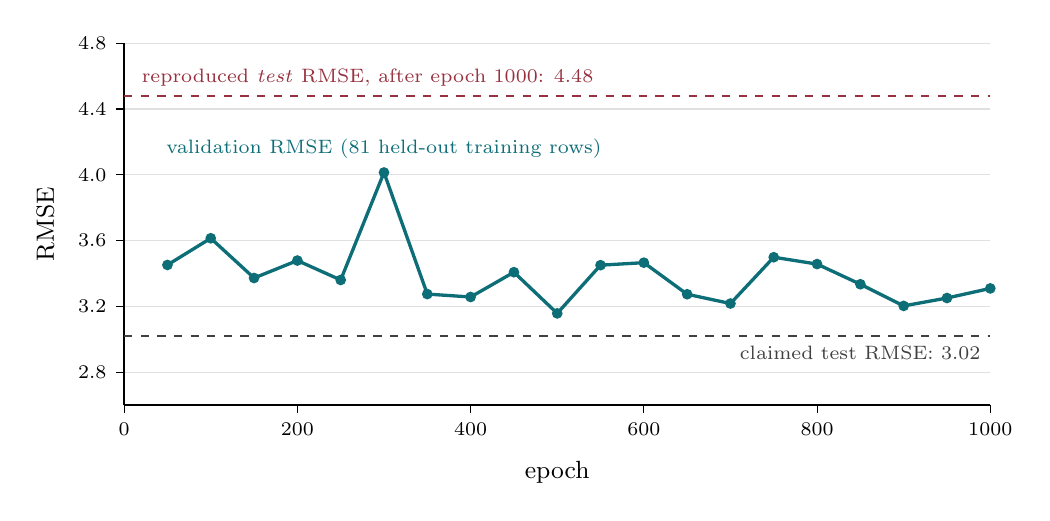
\begin{tikzpicture}[gridc/.style={draw=black!12}]
  \draw (0,0.418) -- (-0.1,0.418) node[left, font=\scriptsize] {2.8};
  \draw[gridc] (0,0.418) -- (11.0,0.418);
  \draw (0,1.255) -- (-0.1,1.255) node[left, font=\scriptsize] {3.2};
  \draw[gridc] (0,1.255) -- (11.0,1.255);
  \draw (0,2.091) -- (-0.1,2.091) node[left, font=\scriptsize] {3.6};
  \draw[gridc] (0,2.091) -- (11.0,2.091);
  \draw (0,2.927) -- (-0.1,2.927) node[left, font=\scriptsize] {4.0};
  \draw[gridc] (0,2.927) -- (11.0,2.927);
  \draw (0,3.764) -- (-0.1,3.764) node[left, font=\scriptsize] {4.4};
  \draw[gridc] (0,3.764) -- (11.0,3.764);
  \draw (0,4.600) -- (-0.1,4.600) node[left, font=\scriptsize] {4.8};
  \draw[gridc] (0,4.600) -- (11.0,4.600);
  \draw (0.000,0) -- (0.000,-0.1) node[below, font=\scriptsize] {0};
  \draw (2.200,0) -- (2.200,-0.1) node[below, font=\scriptsize] {200};
  \draw (4.400,0) -- (4.400,-0.1) node[below, font=\scriptsize] {400};
  \draw (6.600,0) -- (6.600,-0.1) node[below, font=\scriptsize] {600};
  \draw (8.800,0) -- (8.800,-0.1) node[below, font=\scriptsize] {800};
  \draw (11.000,0) -- (11.000,-0.1) node[below, font=\scriptsize] {1000};
  \draw[thick] (0,0) -- (11.0,0);
  \draw[thick] (0,0) -- (0,4.6);
  \node[rotate=90, font=\small] at (-1.0,2.300) {RMSE};
  \node[font=\small] at (5.500,-0.85) {epoch};
  \draw[dashed, draw=missingc, thick] (0,3.931) -- (11.0,3.931);
  \node[font=\scriptsize, text=missingc, anchor=south west] at (0.1,3.931)
    {reproduced \emph{test} RMSE, after epoch 1000: 4.48};
  \draw[dashed, draw=black!75, thick] (0,0.878) -- (11.0,0.878);
  \node[font=\scriptsize, text=black!75, anchor=north east] at (11.0,0.878)
    {claimed test RMSE: 3.02};
  \draw[loopc, very thick, mark=*, mark size=1.3pt]
    plot coordinates {(0.550,1.783) (1.100,2.122) (1.650,1.617) (2.200,1.839) (2.750,1.592) (3.300,2.957) (3.850,1.413) (4.400,1.376) (4.950,1.691) (5.500,1.168) (6.050,1.780) (6.600,1.812) (7.150,1.411) (7.700,1.293) (8.250,1.881) (8.800,1.794) (9.350,1.538) (9.900,1.263) (10.450,1.363) (11.000,1.485)};
  \node[font=\scriptsize, text=loopc, anchor=south] at (3.300,3.007)
    {validation RMSE (81 held-out training rows)};
\end{tikzpicture}
\caption{Wijaya's reproduction at the paper's full setting, from the run log. The model
trained on 324 rows; RMSE on 81 further held-out training rows (every 50 epochs; epoch 1, at
20.7, is off the scale) stayed near the claimed test RMSE throughout, while the 101-row test
set, evaluated once at the end, gave 4.48. Two held-out subsets of the same 506-row dataset
disagree by more than the gap being measured, which is why a single split cannot adjudicate
this reproduction.}
\label{fig:wijaya}
\end{figure}


\textbf{Wijaya.} The reproduced test RMSE of 4.48 is 48\% above the claim, while the
training RMSE of 2.94 is within 9\% of it. The training log qualifies the headline number
(Figure~\ref{fig:wijaya}). The generated script, following the paper's description, held out
20\% of the training rows for monitoring. On those 81 rows, which the model never trained
on, the RMSE stayed between 3.2 and 3.5 for most of training and ended at 3.31 --- close to
the claimed test value. Only the 101-row test set produced 4.48. Two held-out subsets of the
same 506-row dataset thus disagree by more than the gap being measured.

The paper states its split sizes but not how rows were assigned, so the script used a seeded
random split. On a dataset this small, with a target censored at its maximum value, which
rows fall into a 101-row test set plausibly dominates the result. A single seed cannot
separate an unfaithful implementation from an unlucky split, and we do not claim either. Two
further candidates remain untested: the Coder did not reproduce Keras's batch-normalization
and initialization defaults (Section~\ref{sec:findings}), and a constant learning rate left
the final epoch's training loss noisy.

\textbf{SVM guide.} ReproBot reproduced the paper's whole procedure: scale each feature to
$[-1, 1]$ using the training set's ranges, evaluate 110 $(C, \gamma)$ pairs by five-fold
cross-validation, retrain on the full training set with the best pair, and test once. It
reached 96.625\% against the paper's 96.875\%, a difference of 10 of the 4,000 test instances.
The cause is identifiable. The search selected $C = \gamma = 8$ at a cross-validation accuracy
of 96.99\%, where the paper's search selected $C = \gamma = 2$ at 96.89\%. The two candidates
are within a tenth of a point of each other, and which one wins depends on how instances are
assigned to folds, which the paper leaves to its tool's random shuffle. To separate the
implementation from the search, we evaluated scikit-learn's \texttt{SVC} directly at the
paper's settings, outside the pipeline. It reproduced all three of the paper's reported test
accuracies exactly: 66.925\% on unscaled data with default parameters, 96.15\% on scaled data
with defaults, and 96.875\% at $C = \gamma = 2$. Since \texttt{SVC} wraps LIBSVM this is
expected, but it establishes that the reproduction is exact in its implementation and differs
only in one stochastic step of its protocol.

\textbf{Fashion-MNIST random forest.} The five runs gave between 0.8753 and 0.8792, with a mean
of 0.8773 against the claimed 0.873. All five exceed the claim, so the gap of 0.4 points is not
run-to-run noise. Tree ensembles are insensitive to monotonic rescaling of pixel values, so the
unstated preprocessing is an unlikely cause; the scikit-learn version the paper used, also
unstated, is the more plausible one, and we did not isolate it. We read this as a close rather
than an exact reproduction.

\textbf{Soft decision tree.} The generated script had to guess a dozen values the paper does not
state, and disclosed each. After the retry repaired its crash, its three check stages all
passed, yet its accuracy stayed between 5\% and 9\%, below the 10\% of random guessing, and
its training loss was negative and identical to four decimal places across every epoch. That
is a defect in the generated objective rather than slow learning, and the full 40-epoch run
could not change it. The regeneration also silently changed several guessed values --- the
learning rate from 0.01 to 0.1, the batch size from 128 to 32 and the penalty strength from 0.1
to 0.01 --- none of which the triage feedback had asked for. We report no number for this
claim.

\subsection{Cost}

One Coder call consumed approximately 27{,}000 input and 9{,}500 output tokens and took 75\,s;
one triage call, about 2{,}400 input and 240 output tokens, in 3\,s. Compute again dominated,
and in a way worth recording. Both full runs shared the CPU, and each container claimed
every core. Wijaya's 1000 epochs over 324 training rows took 1,906\,s --- about 1.9\,s per
epoch of 11 small batches, which is thread contention rather than model cost --- and Tang's
run took 54 minutes. The Runner deliberately leaves CPU limits unset, because an arbitrary
limit produces failures indistinguishable from crashes; the practical consequence is that
concurrent runs should be avoided.

\section{A Front End: The Pipeline Viewer}
\label{sec:viewer}

In parallel with the pipeline work, the team built ReproBot's first user interface:
\texttt{viewer/}, a dashboard written in Streamlit, developed on a feature branch. The
original proposal planned a Gradio demonstration for the final month; the viewer is an early
step towards it, and is already useful as a working tool.

\textbf{What it shows.} The main page lists every paper with a status table --- whether OCR,
Reader and Coder output exist, and how many validation flags remain. Selecting a paper opens
tabs for its method summary, architecture notes, claims, hyperparameters, data pipeline,
validation flags, raw extraction JSON, generated training script with its
\texttt{reproduce.sh}, and the raw OCR Markdown. A reviewer can therefore inspect what the
Reader extracted and what the Coder did with it side by side, without opening files.

\textbf{What it can run.} An ``Import a paper'' section accepts a PDF upload, with an
optional page limit so that a new paper can be tested cheaply before committing to the whole
document. Per-paper buttons then run Reader extraction or code generation. Two design
decisions make this safe. Every action calls the corresponding stage's own entry point,
unmodified, so the viewer cannot drift from the command-line pipeline. And uploaded papers
are stored in a separate directory rather than the curated dataset directory, which is
maintained by another team member.

\textbf{Status.} The branch was verified with strict type checking, the repository's
pre-commit hooks, and a headless Streamlit run that rendered every tab against synthetic
fixtures. It is not yet merged.
Two gaps remain before it is: it does not yet display Runner or Orchestrator output --- the
results this report is about --- and it predates the generalization of the Coder and Runner,
so its dependency changes need reconciling with the updated lock file before it can merge. Extending it to show a run's attempts, triage decisions and metrics, and
eventually the Critic's verdict, is the natural route to the planned demonstration.

\section{Engineering Findings}
\label{sec:findings}

\subsection{Where the library is the method, exactness is achievable}

The SVM guide shows that some claims can be reproduced exactly, not merely within noise: the
same solver on the same data gives the same number to three decimal places. This sharpens what
a Critic must do. A claim produced by a deterministic library call admits essentially zero
tolerance, and a gap there is diagnostic; a claim produced by stochastic training admits a
tolerance set by run-to-run variance; and a claim like the SVM guide's mixes the two, exact in
its solver and stochastic in its model selection. One tolerance for all claims would be wrong
for most of them.

\subsection{The escalation ladder does not fit models without epochs}

For the random forest and the SVM, \texttt{smoke} and \texttt{capped} produced identical
numbers --- 0.7891 and 94.92\% respectively --- because the two stages differ only in the
number of epochs, which neither model has. For non-iterative models the fourth stage adds cost
and no information; a ladder over training-set size would fit them better.

\subsection{Execution success is not evidence of a result}

Static checks cannot establish that generated code runs; the injected scheduler fault above
parsed cleanly and failed only in execution. This phase established the next step: that code running to completion cannot establish that it
worked. Tang's collapsed run would have exited normally and been reported as a success. The
escalation ladder could not have caught it --- \texttt{capped} trains for about fifteen steps,
and the collapse needed thousands --- and \texttt{capped}'s stated purpose, checking that
training learns, is not enforced by anything: the Runner reads only the exit code.

The soft decision tree repeated the lesson with no scale involved: all three check stages
passed with accuracy below chance and a constant, negative loss. The same pattern appeared at
smaller scale throughout the phase. The \texttt{full} mode of
every generated \texttt{reproduce.sh} wrote its metrics to a different filename from the one
the Runner reads, so both fidelity results above reached the Runner only through its
fallback parser; this is now fixed. The OCR, Reader and Coder stages exit with status zero
even when every paper fails, which is how a missing image-library dependency went unnoticed
on the first OCR attempt of the phase. Every such seam is a place where failure can look like
success.

\subsection{Framework defaults are part of the method}

Two findings point the same way. HuggingFace \texttt{Trainer}'s default gradient clipping
made a script look stable that, written faithfully, diverges. And a paper written in Keras
inherits Keras's defaults wherever it is silent, so reproducing it faithfully in another
framework means reproducing those defaults. The Coder was instructed to do so, and followed
the instruction only partly: Wijaya's script matched Keras's Adam $\epsilon$ but used
PyTorch's batch-normalization momentum and $\epsilon$ and PyTorch's default initialization,
and disclosed the choice rather than following the rule. Disclosure makes a deviation
visible; it does not make it faithful.

\subsection{A remembered identifier is worse than a missing one}

A model that lacks an identifier fails visibly. A model that recalls one wrongly --- a dead
URL, a removed loader, a dataset number one digit away from correct --- produces an artifact
that looks correct and, for a dataset identifier, trains without complaint on the wrong data.
The defence that worked was not asking the model to be more careful, but removing the
opportunity: triage may not name identifiers absent from the log, and the generated script
must verify what it fetched before using it.

\subsection{Prompt wording is executed literally}

The one defect this phase introduced into generated code came from our own prompt, which
described OpenML datasets as pinned by ``data\_id and version''. The description was meant
loosely; the model passed both arguments. Prompts for code generators are read as
specifications, and descriptive phrasing in them needs the same care as an API contract.

\subsection{Unstated values fail jointly}

The Coder's disclosure discipline worked as designed: momentum 0.9 and $C = 1.0$ were both
listed as guesses. What it could not express was that the \emph{combination} was unsafe.
Reporting each unstated value in isolation is necessary but not sufficient; the values that
matter most may be the ones that interact, and finding that out required an ablation. This
argues for recording unstated hyperparameters as carefully as unstated architecture, and
for a cheap automated sensitivity probe over them.

\subsection{One seed cannot adjudicate a gap}

Wijaya's two held-out subsets disagreed by more than the gap between the reproduction and the
claim. A Critic that compares one run against one published number under a fixed tolerance
would declare this reproduction a failure --- and would declare a lucky split a success. A
tolerance must account for the variance of the quantity being compared, which in practice
means several seeds per claim.

\subsection{Regeneration rewrites, measurably}

The retry loop regenerates the whole script on every attempt rather than patching the line at
fault.
Wijaya's repair quantifies the cost: triage's fix was the removal of one keyword argument,
and the regenerated script shared only 22\% of its lines with its predecessor. The repair
succeeded, but almost everything else in the script also changed, unreviewed. The plateau
guard's threshold of 0.98 now has four observations --- 0.41 on the injected scheduler fault and 0.22, 0.25 and 0.27 on real ones --- and none came near it. The soft tree shows the cost
directly: its repair changed three guessed hyperparameters that nobody had asked to change.

\begin{table}[tbp]
\centering
\small
\caption{Status against the project's original four-month plan. \built{} done; \partl{} partial
or in a different form; \absent{} not started.}
\label{tab:timeline}
\begin{tabular}{L{0.1\textwidth}L{0.41\textwidth}cL{0.35\textwidth}}
\toprule
Phase & Planned & & Status \\
\midrule
Month 1 & PDF ingestion; Reader schema; shared-memory object & \built & Complete; five fields \\
Month 2 & Coder and Docker sandbox for a pilot set; Orchestrator skeleton with a single
  hard-coded retry & \built & Exceeded: a bounded retry loop with triage-driven feedback \\
Month 3 & Critic verdict logic & \absent & Not started; first real inputs now exist \\
        & Real retry loop with targeted feedback & \built & Repaired three real defects \\
        & Report Generator & \absent & Not started \\
        & Single-shot vs.\ iterative ablation & \partl & Three observed cases: each fails
  single-shot and runs after one retry \\
Month 4 & Expansion towards 20 papers & \partl & Seven papers across five model families \\
        & Demonstration interface & \partl & Streamlit viewer on a feature branch \\
\bottomrule
\end{tabular}
\end{table}

\section{Development Methodology}
\label{sec:methodology}

ReproBot is built by a human team working with an orchestrating AI coding session, which
delegates scoped tasks to specialized subagents --- research agents that survey precedent,
coding agents that implement and verify a change, review agents that critique an artifact
before a costly action, and validation agents that audit output read-only --- and logs every
delegation with its brief and outcome. Most of this phase's work was investigative rather than
constructive and was carried out directly by the orchestrating session. One scoped implementation --- the generalization of the Coder and
Runner --- was delegated to a coding subagent.

That delegation produced the third instance, across the project, of a subagent's report
being wrong in a way only independent verification caught. The agent reported its
\emph{Network In Network} regression test as a clean pass. It had passed: the script executed
and the metrics file was well formed. The loss was approximately 947. The discrepancy was
found on review, and led directly to the hidden-default finding above. The practice of
treating an agent's report as a claim to check against the diff and the output remains the
most useful single habit we have adopted.

The two most consequential decisions of the phase were human: the direction change to
support multiple task types, and the choice of $C$ for Tang's rerun. The collapse itself was
spotted by a person reading a log. We state this plainly because an automated replication
system is exactly the kind of project in which human intervention can be quietly absorbed
into a result.

\section{Progress Against the Timeline}
\label{sec:timeline}

The project was planned over four months: the Reader in the first; the Coder, sandbox and a
skeleton Orchestrator in the second; the Critic, a real retry loop and the Report Generator in
the third; and evaluation, ablation and a demonstration in the fourth.
Table~\ref{tab:timeline} compares the work to date with that plan. The retry loop arrived ahead of plan and in stronger form than planned. The Critic
and the Report Generator, both Month~3 deliverables, have not started, and the phase's effort
went instead to generalization and to obtaining the first measurable results --- a trade we
consider correct, since a Critic without measurable results would have had nothing to judge.


\section{Limitations}
\label{sec:limitations}

\textbf{The fidelity results are compared by hand, mostly from single runs.} Only the random forest reports a spread over runs, and no stage of the system performed any
comparison.

\textbf{Model-family coverage is still narrow.} No gradient-boosting library (XGBoost, LightGBM,
CatBoost), sequence model, graph network or text model has yet been run, and one model family,
the soft decision tree, produced no result at all.

\textbf{Tang's positive result required a human.} Tang's reproduction matches its claim only
after a person chose one hyperparameter, informed by an ablation that had logged test error.

\textbf{The negative result is not attributed.} Wijaya's gap may stem from the unstated
split, from framework defaults the Coder did not reproduce, or from the implementation, and
one seed cannot distinguish them.

\textbf{The CIFAR-10 benchmark remains unmeasured.} GPU compute is still required for it, and
the two CPU-sized papers are not substitutes for the planned evaluation, only a way to test
the pipeline's claim end to end.

\textbf{The Reader does not record missing hyperparameters}, and claims are duplicated
across a paper's prose, tables and figures. Validation still does not converge, and two of
the eight CIFAR-10 papers still cannot be extracted.

\textbf{A note on the dataset.} Boston Housing includes a feature derived from the
proportion of Black residents in each town \cite{harrison1978hedonic}, which is among the
reasons scikit-learn deprecated and then removed its loader. We used it only because the paper
under replication did, and do not recommend it for any other purpose.

\section{Next Steps}
\label{sec:next}

\textbf{Build the Critic, with variance in mind.} Its verdict should remain explicit
arithmetic against a numeric tolerance using the claim's direction, as planned; Wijaya shows
that the tolerance must be informed by several seeds per claim rather than one run. Tang's
collapsed run is its first test case: a verdict of \emph{fail} at 89\% error against 0.87\%
is the minimum it must deliver.

\textbf{Make the Runner check that training learns.} Reading \texttt{train\_metric} at
\texttt{capped}, and comparing a run's loss against the trivial input-ignoring floor, would
have flagged Tang's collapse within twenty epochs. This is smaller than the Critic and
catches a different failure.

\textbf{Record and probe unstated hyperparameters.} Extend the Reader's gap-recording to
hyperparameters, and automate what the Tang ablation did by hand: short runs over candidate
values for the unstated ones, selected on training health and a validation split --- never
the test set.

\textbf{Patch rather than regenerate.} A line-range edit, as in AutoReproduce
\cite{zhao2025autoreproduce}, would keep a one-argument fix to one argument.

\textbf{Fit the escalation ladder to the model.} Scale training-set size rather than epochs
for non-iterative models, and reject a check stage whose loss does not move.

\textbf{Widen coverage.} Run the diversity targets already selected --- gradient-boosting
libraries, a graph convolutional network, a text CNN and a temporal convolutional network ---
which requires adding XGBoost, LightGBM and CatBoost to the sandbox image.

\textbf{Merge and extend the viewer} to show Runner, Orchestrator and Critic output, as the
basis of the final demonstration.

\textbf{Secure GPU compute} for the CIFAR-10 set, and build the Report Generator and a
single entry point from PDF to report, after fixing the stages that exit successfully on
failure.

\section{Conclusion}
\label{sec:conclusion}

This phase produced ReproBot's first replication measurements, across five papers and five
model families. Three reproductions land close to their claims, one of them exact in its
implementation; one misses its claim by a margin a single split cannot explain; and one never
learned. Getting there required generalizing the pipeline beyond image classification and
beyond neural networks, turning six real prompt failures into explicit rules, and diagnosing a
training collapse that every stage of the pipeline reported as a success.

That last point is the phase's main result, and it happened twice. ReproBot can now read a
paper, write an implementation in the right library, execute it at the paper's own scale, and
repair its own execution failures. What it cannot yet do is tell whether the number it produced
is right. Every measurement in this report was judged by people, and one of them needed a
person to fix it first. Building the component that makes those judgements automatically ---
with a tolerance that respects whether a claim is deterministic or stochastic --- is the work of
the next phase.

\bibliographystyle{plain}
\begin{thebibliography}{9}

\bibitem{tang2013dlsvm}
Tang, Y. (2013).
Deep Learning using Linear Support Vector Machines.
\textit{ICML 2013 Workshop on Challenges in Representation Learning}. arXiv:1306.0239.

\bibitem{wijaya2023housing}
Wijaya, R. (2023).
Multi Level Dense Layer Neural Network Model for Housing Price Prediction.
\textit{arXiv:2310.08133}.

\bibitem{harrison1978hedonic}
Harrison, D., \& Rubinfeld, D.~L. (1978).
Hedonic housing prices and the demand for clean air.
\textit{Journal of Environmental Economics and Management}, 5(1), 81--102.

\bibitem{hsu2003guide}
Hsu, C.-W., Chang, C.-C., \& Lin, C.-J. (2003).
A Practical Guide to Support Vector Classification. Technical report, Department of Computer
Science, National Taiwan University (version updated 2025).

\bibitem{chang2011libsvm}
Chang, C.-C., \& Lin, C.-J. (2011).
LIBSVM: A library for support vector machines.
\textit{ACM Transactions on Intelligent Systems and Technology}, 2(3), 27.

\bibitem{xiao2017fashion}
Xiao, H., Rasul, K., \& Vollgraf, R. (2017).
Fashion-MNIST: a Novel Image Dataset for Benchmarking Machine Learning Algorithms.
\textit{arXiv:1708.07747}.

\bibitem{pedregosa2011sklearn}
Pedregosa, F., Varoquaux, G., Gramfort, A., et al. (2011).
Scikit-learn: Machine Learning in Python.
\textit{Journal of Machine Learning Research}, 12, 2825--2830.

\bibitem{frosst2017soft}
Frosst, N., \& Hinton, G. (2017).
Distilling a Neural Network Into a Soft Decision Tree. \textit{arXiv:1711.09784}.

\bibitem{zhao2025autoreproduce}
Zhao, X., Sun, M., Wang, W., et al. (2025).
AutoReproduce: Automatic AI Experiment Reproduction with Paper Lineage.
\textit{arXiv:2505.20662}.

\end{thebibliography}

\end{document}
